\subsection{ Zr($10\bar{1}0$) surface.}
\begin{frame}{ Zr($10\bar{1}0$) surface, Oxygen and Hydrogen Absorption}

\begingroup
\small
  This project is carried on in colaboration with Fernando Soto, a Postdoc at 
  Perla Balbuena's group in Texas A\&M University, USA. 
\endgroup
  \begin{block}{Progress so far}
  \begin{itemize}
      \item<1-> Oxygen Coverage with alloy elements
	\begin{columns}<1>
	  \column{0.3\textwidth}<1>
	\vspace{1cm}
	  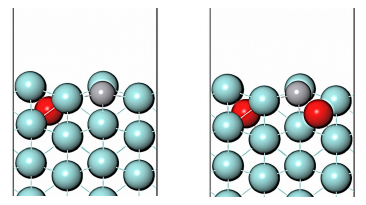
\includegraphics[width=\textwidth]
	  {/home/mariano/CuadernoTrabajo/CV/SLI/02-CurrentResearch/coverage.png}<1>
	  \column{0.7\textwidth}<1>
	\vspace{1cm}
	  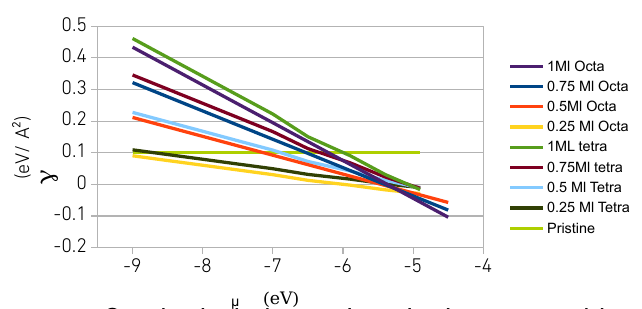
\includegraphics[width=\textwidth]
	  {/home/mariano/CuadernoTrabajo/CV/SLI/02-CurrentResearch/SurfaceEnergies.png}<1>

%	\begin{center}
%	  \includegraphics[height=3.5cm,trim={1cm 16.5cm 5cm 3cm},clip]
%	  {./02-CurrentResearch/OxygenBindingEnergy.pdf}<1>
%	  }$
%	\end{center}
	\end{columns}
      \item<2> AIMD: Hydgrogen moves differently in the presence of Ta and V,

	\begin{columns}
	  \column{0.6\textwidth}
	  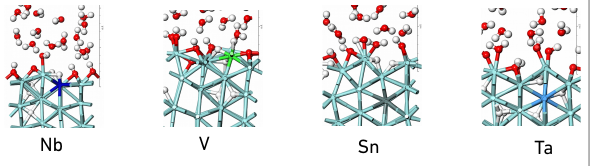
\includegraphics[width=\textwidth]
	  {/home/mariano/CuadernoTrabajo/CV/SLI/02-CurrentResearch/Alloys-AIMD.png}<2>
	  \column{0.4\textwidth}
	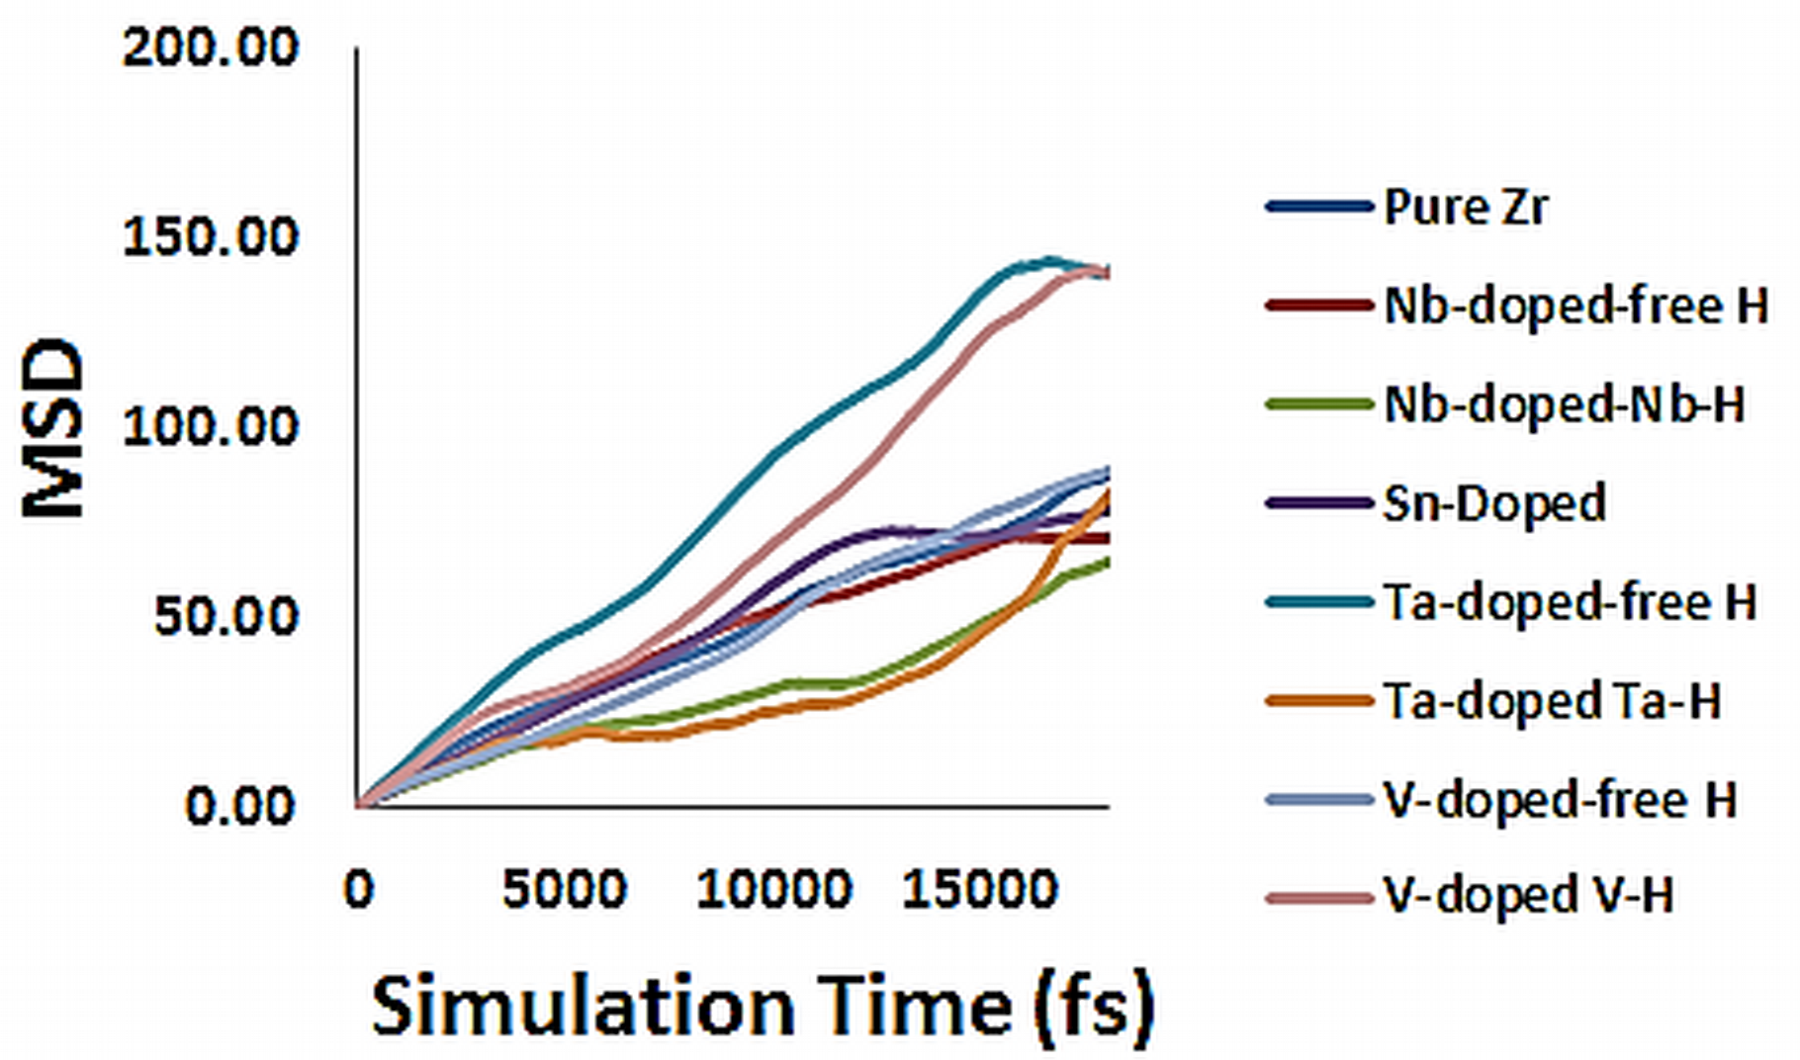
\includegraphics[width=\textwidth]{./02-CurrentResearch/HydrogenMeanFreePaths.png}<2>
	\end{columns}
  \end{itemize}
  \end{block}

\end{frame}
